%%%%%%%%%%%%%%%%%%%%%%%%%%%%%%%%%%%%%%%%%
% a0poster Portrait Poster
% LaTeX Template
% Version 1.0 (22/06/13)
%
% The a0poster class was created by:
% Gerlinde Kettl and Matthias Weiser (tex@kettl.de)
% 
% This template has been downloaded from:
% http://www.LaTeXTemplates.com
%
% License:
% CC BY-NC-SA 3.0 (http://creativecommons.org/licenses/by-nc-sa/3.0/)
%
%%%%%%%%%%%%%%%%%%%%%%%%%%%%%%%%%%%%%%%%%

%----------------------------------------------------------------------------------------
%	PACKAGES AND OTHER DOCUMENT CONFIGURATIONS
%----------------------------------------------------------------------------------------

\documentclass[a0,portrait]{a0poster}

\usepackage{subcaption} 

\usepackage{ wasysym } % astrosun symbol.
\usepackage{gensymb} % degree symbol
\usepackage{multicol} % This is so we can have multiple columns of text side-by-side
\columnsep=100pt % This is the amount of white space between the columns in the poster
\columnseprule=3pt % This is the thickness of the black line between the columns in the poster

\usepackage[svgnames]{xcolor} % Specify colors by their 'svgnames', for a full list of all colors available see here: http://www.latextemplates.com/svgnames-colors

%\usepackage{times} % Use the times font
\usepackage{palatino} % Uncomment to use the Palatino font

\usepackage{graphicx} % Required for including images
\graphicspath{{figures/}} % Location of the graphics files
%\usepackage{booktabs} % Top and bottom rules for table
\usepackage[font=small,labelfont=bf]{caption} % Required for specifying captions to tables and figures
%\usepackage{amsfonts, amsmath, amsthm, amssymb} % For math fonts, symbols and environments
\usepackage{wrapfig} % Allows wrapping text around tables and figures
\usepackage{url}

%\usepackage{realboxes}

\renewcommand{\emph}[1]{\textbf{\color{blue}#1}}

\newcommand{\vs}[1] {\textbf{\textcolor{red}{#1}}}

\newcommand{\ECM}[1] {\textbf{\textcolor{magenta}{#1}}}

%\renewcommand{\section}[2]{\Colorbox{lightgray}{\noindent {\Large \textbf{#2}} \hfill}}

%\usepackage{lipsum}

\begin{document}

%----------------------------------------------------------------------------------------
%	POSTER HEADER 
%----------------------------------------------------------------------------------------

% The header is divided into two boxes:
% The first is 75% wide and houses the title, subtitle, names, university/organization and contact information
% The second is 25% wide and houses a logo for your university/organization or a photo of you
% The widths of these boxes can be easily edited to accommodate your content as you see fit

\begin{minipage}[b]{0.75\linewidth}
  \Huge \textbf{Prospects about X- and gamma-ray counterparts of gravitational-wave signals with INTEGRAL}\\[1cm] % Title
  \large \textbf{P.~Bacon, V.~Savchenko and E.~Chassande-Mottin}\\[1cm] % Author(s)
  \normalsize APC, Univ Paris Diderot, CNRS/IN2P3, CEA/Irfu, Obs. de Paris, Sorbonne Paris Cit\'e, France\\
  \large \texttt{philippe.bacon@apc.in2p3.fr}\\
\end{minipage}
%
\begin{minipage}[b]{0.25\linewidth}
	
\includegraphics[scale=.8]{logo.png}
\end{minipage}

\vspace{1cm} % A bit of extra whitespace between the header and poster content

%----------------------------------------------------------------------------------------

\begin{multicols}{2} % This is how many columns your poster will be broken into, a portrait poster is generally split into 2 columns


 \begin{abstract}
   By extrapolating the number of detections made during the first LIGO science
   run, tenths of gravitational wave signals from binary black hole mergers are
   anticipated in upcoming LIGO Virgo science runs. Finding an electromagnetic
   counterpart to compact binary merger events would be a landmark
   discovery. The search for such counterpart is challenging for a number of
   reasons, such as the poor resolution of source position reconstruction from
   the gravitational wave observations alone, and the weakness of the expected
   electromagnetic signal. In this poster, we evaluate the ability of current
   wide-field X- and gamma-ray telescopes aboard INTEGRAL to find such
   counterparts. We present the result of an end-to-end simulation for
   estimating the fraction of the sources that can be followed up, and the
   fraction of counterparts that can be detected based on different models.
 \end{abstract}

 % satellite : What fraction of GW events can be recovered in the EM spectrum ?
 % What should be the statistical significance of the GW and the EM events to
 % claim a confident joint detection ? \textcolor{blue}{BOTTOM LINE RESULTS : We
 % show that...}

\section*{Motivations}

\ECM{Intro on LIGO Virgo -- Objective of the study and major steps. Follow-up 
campaing during O1. Constraints set by INTEGRAL on GW150914 \cite{2041-8205-820-2-L36}}

\emph{We produce a end-to-end simulation of the search for gravitational-waves
from binary neutron star mergers \textit{and} follow-up observation seeking a
 possible electromagnetic counterpart at high-energies.} This study is similar
to the one done in \cite{2016arXiv160606124P} with Fermi.

\section*{Monte-Carlo simulation of gravitational-wave events from neutron-star binary mergers}

We start with a simulated catalogue of 6 millions Milky Way-like galaxies
distributed to $z\sim 0.12$. To those galaxies, we associate binary neutron star
(BNS) mergers with mass distribution and rate of R=$23.5 M\mathrm{yr}^-3$ per galaxy
according to Model A ($Z_{\astrosun}$ metallicity) of
\cite{dominik12:_doubl_compac_objec}. This results in a population of 14\,000
mergers for a $100$ year simulation.

\begin{center}\vspace{.5cm}
    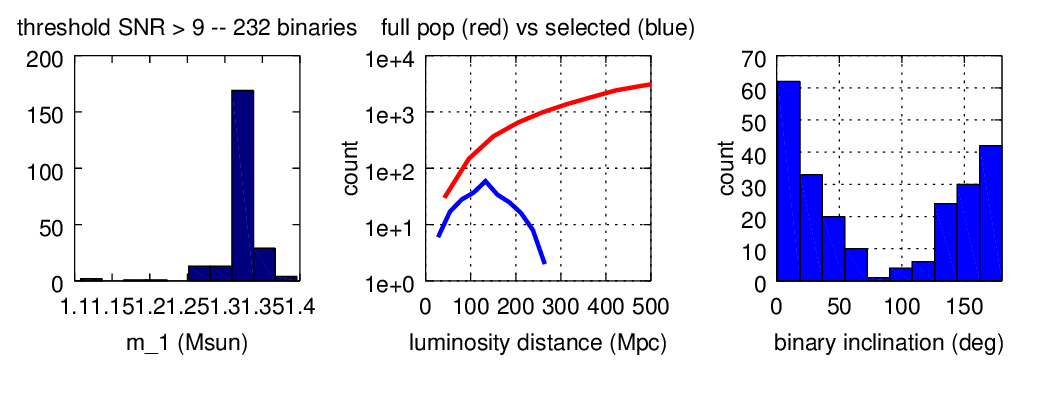
\includegraphics[width=30cm]{figures/summary_plot.png}
    %\includegraphics[width=30cm]{figures/}
\end{center}

We inject GW signals corresponding to the binary mergers (using model
``TaylorT4'') and inject them into Gaussian noise colored according to the
``optimistic'' power-spectral density anticipated for the 2nd LIGO/Virgo run O2
\cite{lrr-2016-1}. We select signals with $\mathrm{SNR}_{\mathrm{combined}} > 9$
corresponding to a false-alarm rate $\mathrm{FAR} < 1/\mathrm{month}$. The average range
BNS is 126 Mpc for this selection.

This results in 232 selected merger signals over 100 years which corresponds to
$\sim 1$ merger over the 6-month duration of O2. We distribute those events randomly in
time over the expected period of O2 from Nov 2016 to May 2017. We
recover GW signals using matched-filtering techniques and reconstruct the
posterior skymaps giving the position of the source with the BAYESTAR pipeline
\cite{PhysRevD.93.024013}.

\ECM{XXX add typical size of search area -- say poorly resolve XXX}


% SNR threshold HL = 6 : RHO_thres_NETWORK = sqrt(rho_H**2 + rho_L**2) = 6
% On one hand, the signal only takes the inspiral phase into account via the use of non-spinning waveform 'TaylorF4ThreePN'.
% As we want to reproduce an analogue study with \textsc{INTEGRAL} it justifies why our simulation settings are aligned on their work. This will allow further comparisons.
% As a transition towards the details of the EM emission we estimated the total GW emitted energy $E_{\mathrm{EM}}$ of the simulated BNS systems thanks to Bernuzzi et al. \cite{2016PhRvD..94b4023B}, ie.  $E_{GW} \sim 1.5 \% \, M c^{2}$ where M is the total mass of the binary.

\section*{Electromagnetic emission model from neutron-star binary mergers}

\ECM{Tell: Connection BNS / Gamma-ray bursts, simplified GRB emission model with basic features}

Every simulated GW event is associated to a gamma-ray event.

Observational evidences of GRBs generally show two kinds of EM emissions : a
prompt emission in the gamma-ray or X-ray domain which corresponds to the
collimated ejection of relativistic jets of matter, and an afterglow emission in
the X-ray, optic or radio domain produced after the ejecta has been slowed down
by internally driven shocks between many layers.

\subsection*{Prompt emission}

\ECM{Tell: light curve evolution, isotropic emitted energy and beaming}

The prompt emission is well modelled by the BAND emission spectrum with the
following fixed parameters $\alpha_{\mathrm{BAND}} = - 0.5$,
$\beta_{\mathrm{BAND}} = - 2.25$ and $E_{\mathrm{peak}} = 800 \, MeV$. As it is
associated to the coalescence of the BNS it is not expected to last more than a
few seconds. 

\subsection*{Afterglow}

\ECM{Tell: light curve evolution, isotropic emitted energy and beaming}

As well the afterglow emission in the X-ray lasts until 3 days after the
coalescence of the BNS system and is modelled by a cut-off power law with
$\lambda = - 0.5$ and $E_{\mathrm{peak}} = 600 \, keV$. 

% Power law model see Eq(1) of 'THE FERMI GBM GAMMA-RAY BURST SPECTRAL CATALOG: FOUR YEARS OF DATA' - Gruber et al 

\begin{center}\vspace{.5cm}
    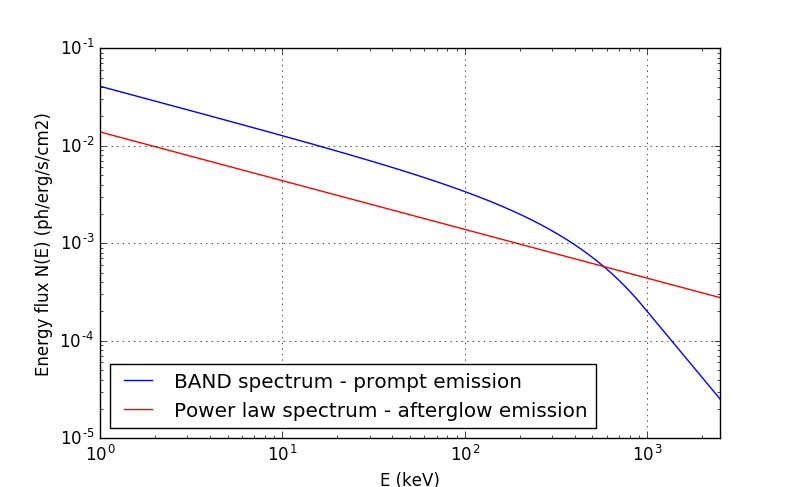
\includegraphics[width=20cm]{figures/spectra.png}
    \captionof{figure}{Prompt and afterglow emission spectra from SGRBs systems. Fluxes have been normalized with respect to the INTEGRAL finite energy band $\left[ 75 \, , 2000 \right] \, \mathrm{keV}$.}
    \label{spectra}
\end{center}

\section*{The INTEGRAL mission and possible follow-up strategies}

\ECM{Volodymyr: Describe the relevant instruments here. Energy range covered. FOV. 
Graphical scheme of the instrument? Tell the two possible follow-up strategies}

The INTEGRAL satellite embarks the SPI-ACS gamma-ray spectrometer and the IBIS
imager. The former takes advantage of a very wide field of view (FoV) essential
to monitor prompt emissions (passive follow-up) whereas the latter has a good
spatial resolution once is is on source (active follow-up).

The afterglow emission being of longer duration, it allows to re-point the
INTEGRAL satellite and to align the IBIS instrument onto the source.

% As GRBs will then be monitored thanks to the SPI-ACS and IBIS instruments embarked on the \textsc{INTEGRAL} satellite mission, we thus have to convert the energy information into some constraints acting on the detectable energy flux by those instruments. The emitted EM flux is hence truncated to the \textsc{INTEGRAL} finite energy band $\left[ 75 \, , 2000 \right] \, \mathrm{keV}$. \\

\begin{center}
    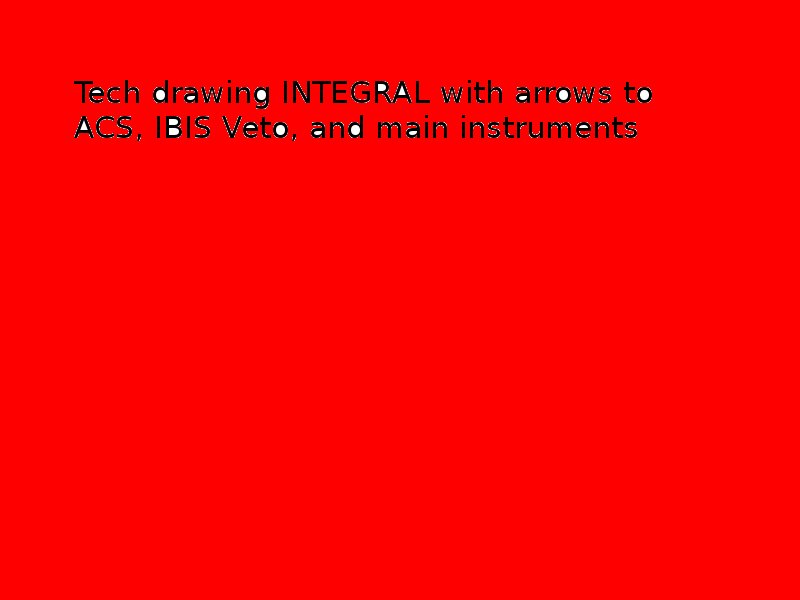
\includegraphics[width=10cm]{figures/INTEGRAL.png}
\end{center}

\section*{Results}

\subsection*{Passive follow-up of prompt emission}

\begin{center}
    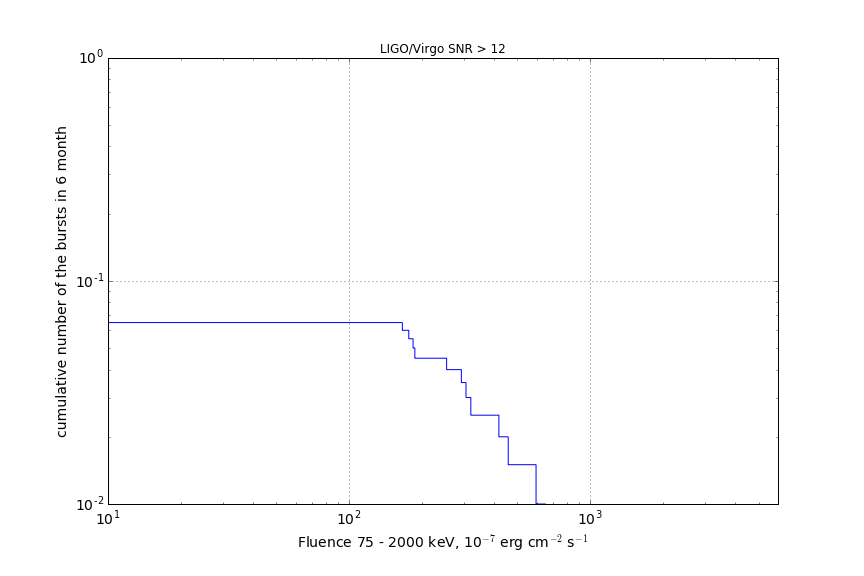
\includegraphics[width=11cm]{figures/fluence_distribution_12.png}
 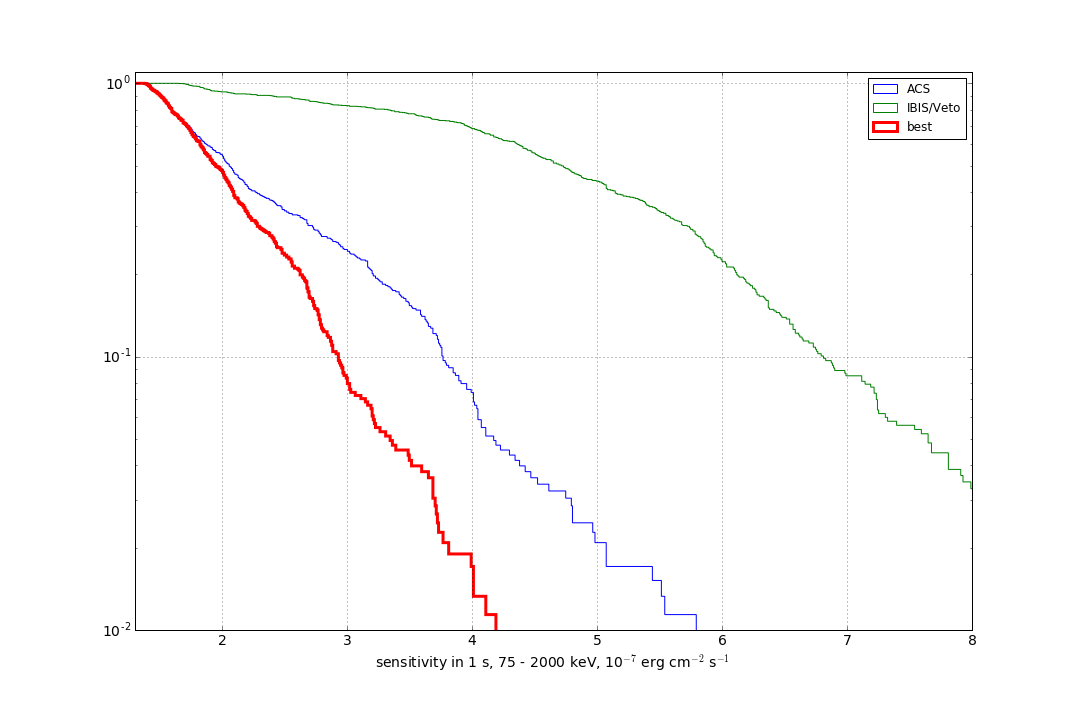
\includegraphics[width=11cm]{figures/sensitivity_distribution.png}
    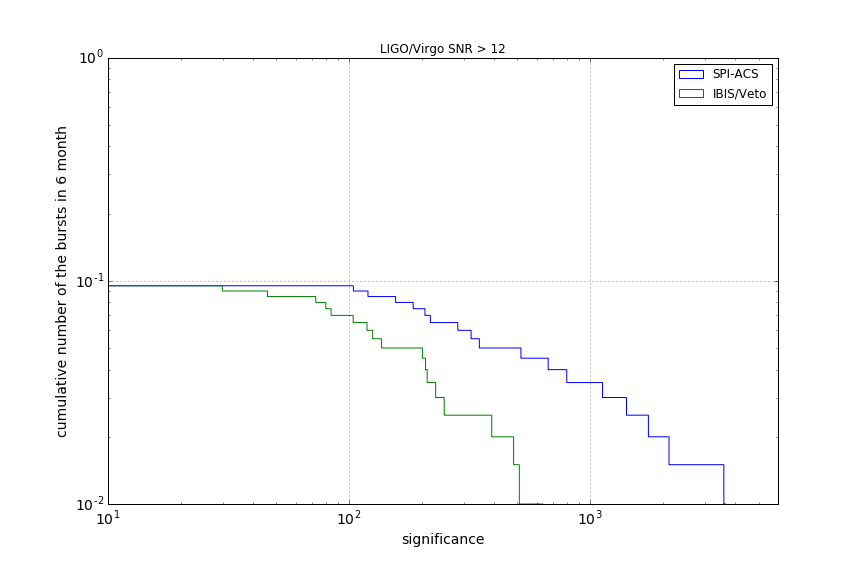
\includegraphics[width=11cm]{figures/significance_distribution_12.png}
    \captionof{figure}{}
\end{center}

The fluence of the prompt emission associated to GW alerts is in the range
$150--600 \times 10^-7$ erg cm$^{-2}$s$^{-1}$. This is much brighter than the
limiting flux from SPI-ACS. Note the better sensitivity when combined with
IBIS/Veto thanks to the complementarity of their field of view.  

\ECM{Volodymyr, is the following true?}

SPI-ACS detects with high significance $> 100 \, \sigma$ the prompt emission of
all 4-sigma events oriented towards the detector within the beaming angle.

\ECM{Volodymyr, please fill the XX}

SPI-ACS and IBIS/Veto allows to follow XX \% of the alerts with a 
$XX \, \sigma$ significance.

\subsection*{Instrument repointing to follow afterglows}

\ECM{Volodymyr, it is not clear in your notes what instrument (IBIS?) is being
  used here. Can you specify? What is the ``currently assumed follow-up
  strategy''?}

\ECM{Volodymyr, what's the curve in blue in the covered region plot? In the same
  plot, would be better to see distribution relative to all $SNR > X$ events --
  saturate to 1 on the left.}

\begin{center}
    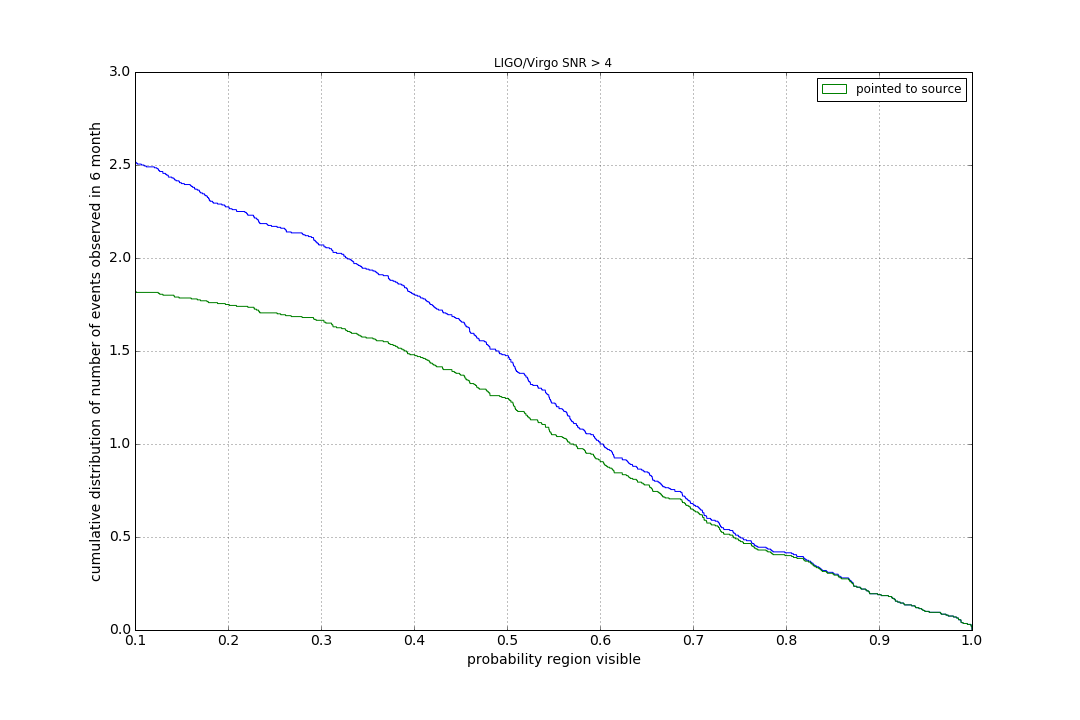
\includegraphics[width=11cm]{figures/covered_region_4-1.png}
    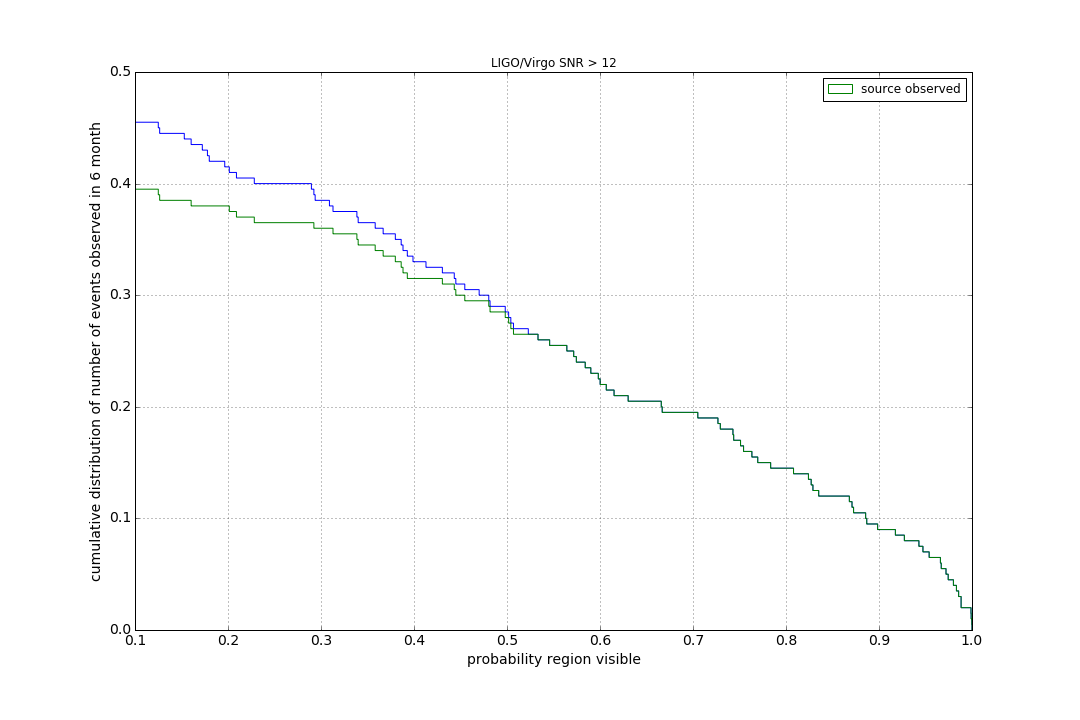
\includegraphics[width=11cm]{figures/covered_region_12-1.png}
    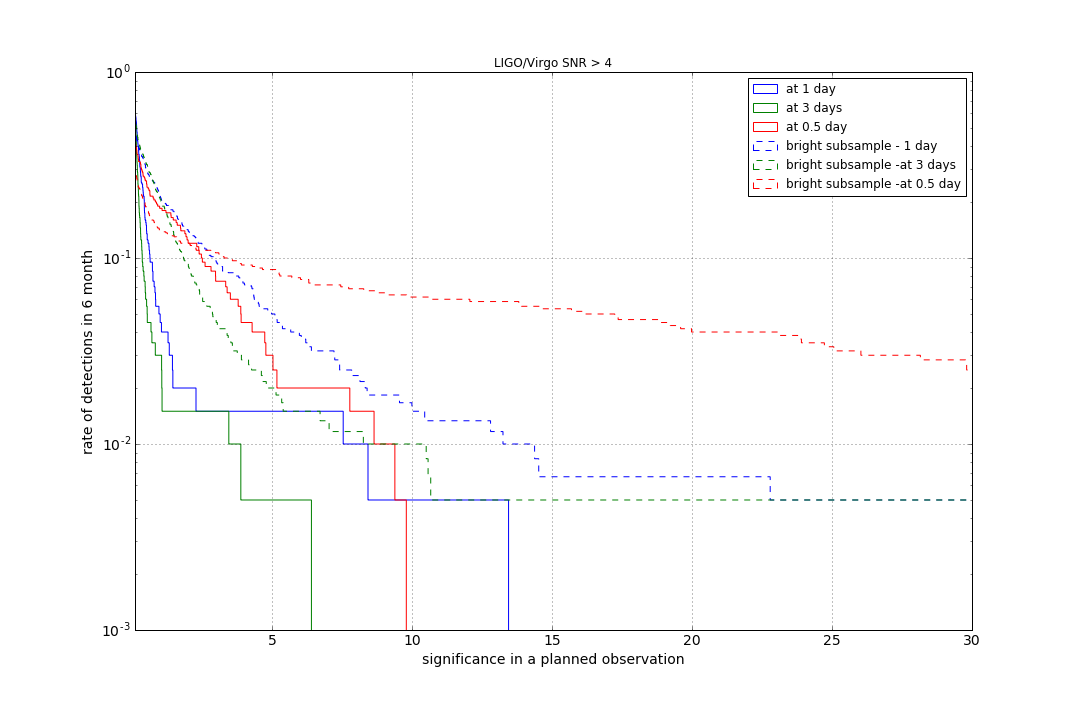
\includegraphics[width=11cm]{figures/ag_flux_4.png}
    \label{covered_region}
\end{center}

The fraction of the region accessible for pointed follow-ups is larger than The
error-box area covered by INTEGRAL. We can trigger a follow-up if more than 30
\% of the error box is initially covered.

\ECM{Volodymyr, what are the conclusions here?}

% \section*{Conclusions}

% Among compact objects populations GRBs are the most promising astrophysical
% sources from which we can expect a gamma-ray emission loud enough to be
% associated to GW radiation sources and thus be detectable with adequate
% instruments. We show in this poster that INTEGRAL is the appropriate to ensure a
% follow-up for both the prompt and afterglow emissions, thanks to the IBIS and
% SPI-ACES instruments.

%----------------------------------------------------------------------------------------
%	ACKNOWLEDGEMENTS
%----------------------------------------------------------------------------------------

\vspace{10mm}
\noindent {\normalsize \textbf{Acknowledgements}}

{\footnotesize 
  This research was supported in part by the ASTERICS grant. The authors would like to thank Barbara Patricelli for sharing data and Philippe Laurent for fruitful discussions. }
  %We thank ASTERICS. Barbara Patricelli for sharing data, Philippe Laurent for discussions}

%----------------------------------------------------------------------------------------
%	REFERENCES
%----------------------------------------------------------------------------------------

%\nocite{*} % Print all references regardless of whether they were cited in the poster or not
\bibliographystyle{plain} % Plain referencing style
\bibliography{reference} % Use the example bibliography file sample.bib

%----------------------------------------------------------------------------------------

\end{multicols}
\end{document}
